% Chapter X

\chapter{Multi-source detection of complex anomalies} % Chapter title
\label{ch:joint} % For referencing the chapter elsewhere, use \autoref{ch:name} 
\minitoc% Creating an actual minitoc\
\bigskip

In the previous chapters, we presented methods for anomaly detection related to each of the observability components. However, as standalone detectors from the corresponding data source, they have a limited view on the system. In this regard, insights gleaned from a combination of different observability signals are necessary to properly troubleshoot distributed systems~\cite{sridharan2018distributed}.

In this chapter, we analyze whether the full observability of the system, i.e., recording metrics, logs, and traces, provides exposure of the broader spectrum of anomalies. The contributions presented in this chapter are summarized below~\footnote{Parts of this chapter are published in ~\cite{nedelkoski2020data,nedelkoski2020jointmodalities,nedelkoski2019distributions}.}. 

\begin{itemize}
    \item We provide an analysis of complex anomalies in distributed software systems and their reflection in the observability components.
    \item A heuristic for detection of one of three system health states (normal, degradation, and failure state) is described by utilizing the data sources affected by an anomaly.
    \item By presenting case studies of complex anomalies, we show that a rule-based integration of the anomaly detectors helps broaden the spectrum of possible anomalies that can be detected. 
    \item We open-source the testbed and multi-source data, available on Zenodo~\footnote{https://zenodo.org/record/3549604}.
\end{itemize}

\section{Complex anomalies in distributed systems}
Often referenced reasons in various failure analysis studies on distributed software systems are attributed to deployments, exceeding scaling limits, infrastructure changes, and various system and software failures~\cite{sillito2020failures}. We relate them with the properties of the  distributed systems, particularly with the heterogeneity, scalability, and concurrency. 

The heterogeneity in the distributed systems implies complex pieces of code that stick together different resources, written in potentially different programming languages. Consequently, software bugs are unavoidable. Often, in software upgrades, a small configuration change in a system component can be overlooked. This can lead to failures of the system component. As the components (e.g., services) in a distributed system communicate through the network, it is highly likely that the anomaly will affect other system components. 

Prior to the system deployment in production, numerous tests are executed to evaluate the functionality of the system, e.g., under various loads. However, particular limits of the system are infeasible to be tested. Exceeding the scaling limits is one of the causes for failures in the systems. Examples include the rapid increase in the number of concurrent user requests. It can be to a point where a component of the system is not scalable or a system may exhaust available resources, which
implies a resource leak. Thus, the concurrency and scaling of distributed software systems can strongly influence the appearance of complex anomalies.

\begin{figure}[!t]
\centerline{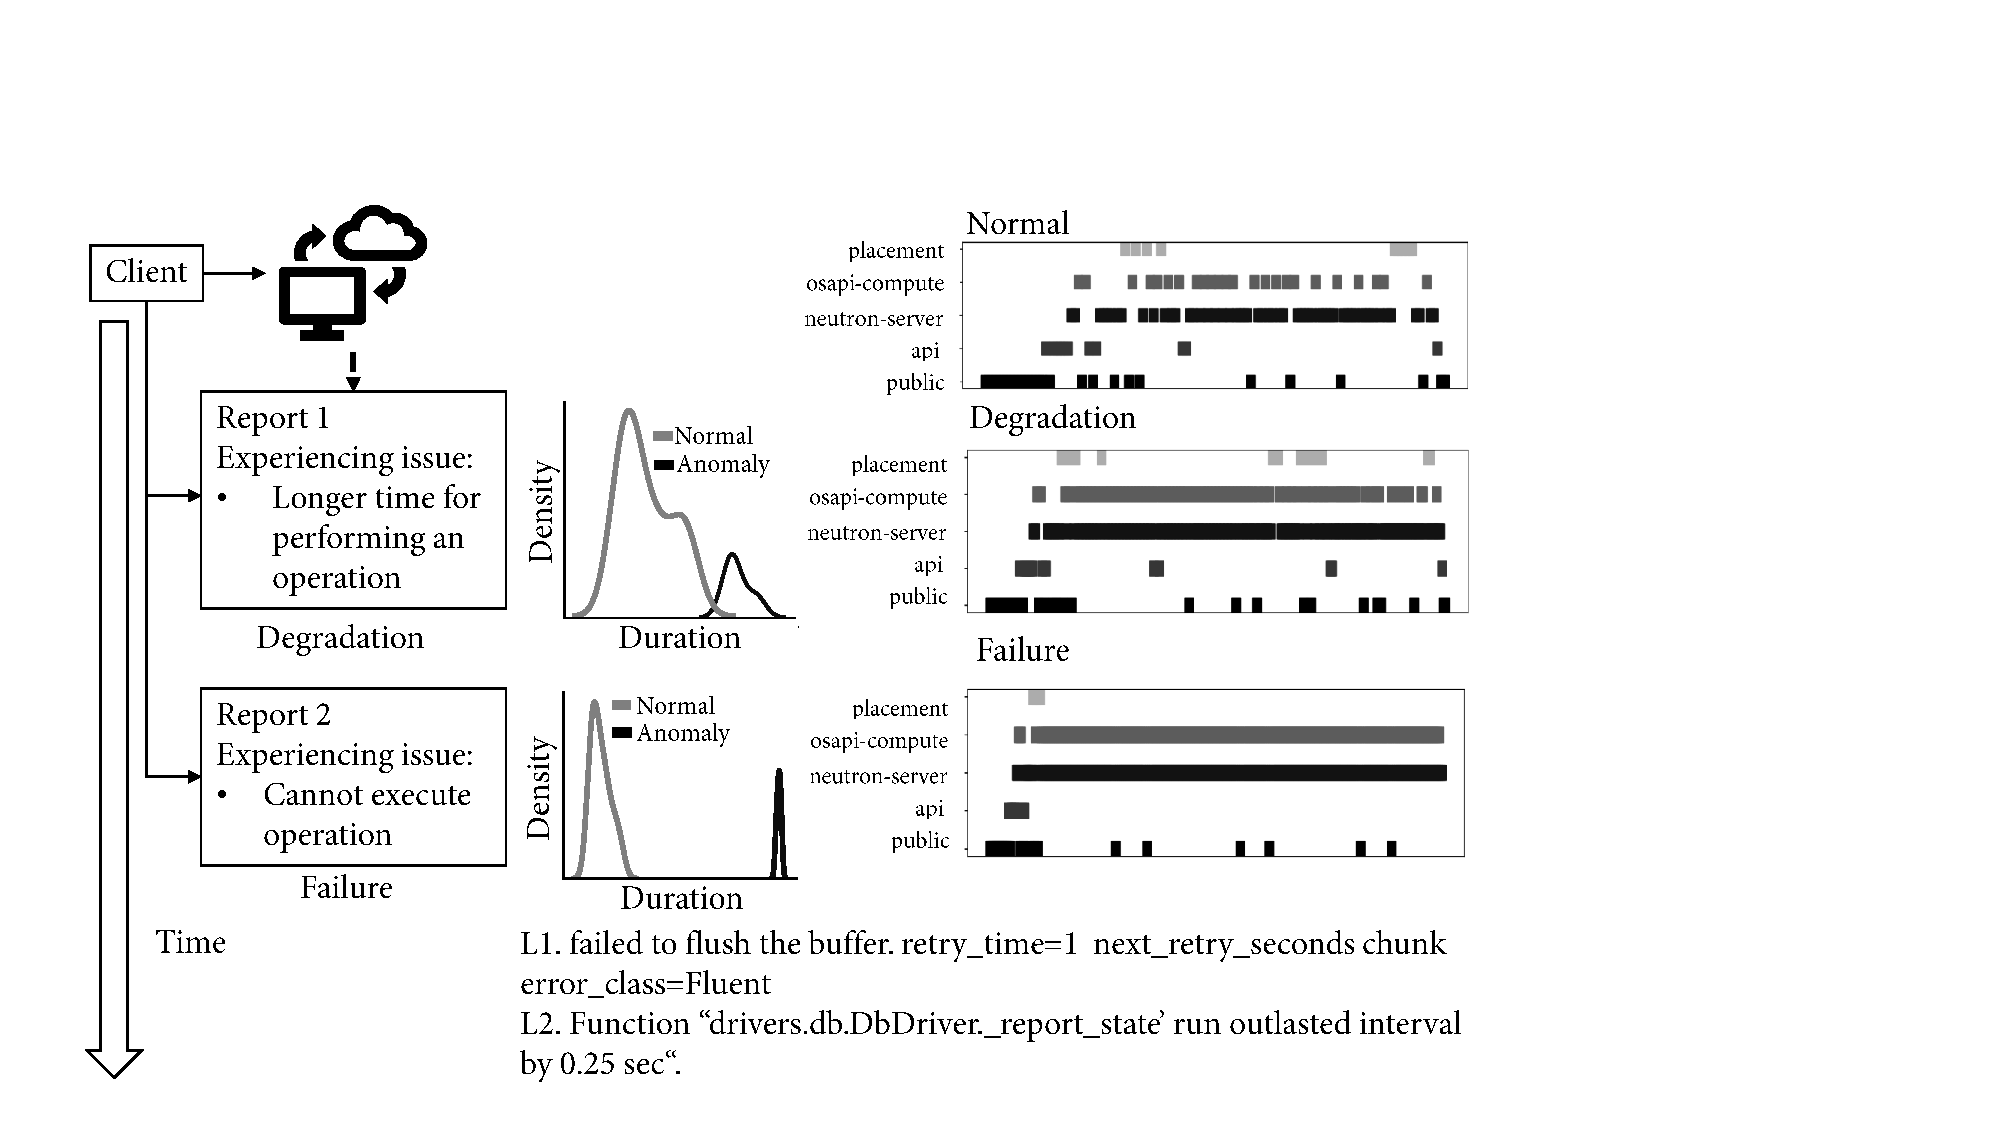
\includegraphics[width=1.0\textwidth]{gfx/chap7/complexanomalies.pdf}}
\caption{Complex anomalies in the Openstack use case.}
\label{fig:complexanomalies}
\end{figure}

The analyzed complex anomalies are anomalies that do not reflect in each of the observability data. For example, a possible anomaly could not be (or hardly) observed in metrics, but easily found in the logs. In the following use-case, we perform an experiment where specific anomalies are reflected only in different data sources. We consider a scenario as in Figure~\ref{fig:complexanomalies}, where the anomaly is originated from the failure in the networking infrastructure on a hardware level, which eliminates the access to the compute host. This anomaly propagates on a application level, where services are affected. Mainly the compute host is responsible for the creation of VMs. Depending on the severity of the problem of the networking infrastructure, the system will be in a degraded or failure state of operation, i.e, the compute service will have a decreased performance or will not be reachable. The right panel shows the metrics, logs, and traces. The top right image presents a model of a trace generated during the normal operation of the system and serves as a nominal value for comparison to the rest of the scenarios (degraded and failure). The plots in the center in gray show the normal distributions of the duration for performing the operation. The anomalous distribution times are presented in black. We assume that the operator has trained anomaly detectors available for all system data sources.

Over time, the client experiences a time of creation of VM longer than usual. However, the client files the first report stating "Longer time for performing an operation". The operator analyzes this report, consults the anomaly detector on the response time, and finds that the response time is larger. However, the observed response time value is in the overlap of the distributions of normal and abnormal duration times. The operator is not sure if he/she should implement further actions. If trace anomaly detection is available to the operator, he/she can immediately observe that the trace is structurally different, compared to the structure when the trace is normal. These differences can be visually observed in Figure~\ref{fig:complexanomalies}. 
The timely observation allows the operator to notice and react to an anomaly during the degraded state of the system. If the operator at this point in time consults the logs, no issue will be reported. This anomaly is not reflected in the structure of the logs, as the operation finishes successfully. Therefore, having the multiple perspectives of the system at disposal provides a higher visibility and supports the correction of false or uncertain predictions reported by a single model. In this case, the trace suggests an anomaly, while the anomaly is not easily observed in the logs and metrics.

In second case, the client issues another report stating "Cannot execute any operation". The consulting of the three modalities then clearly shows a failure, compared to the previous case of degraded state. In addition, according to the trace, most likely, the problem is in the api service as it cannot be contacted. This problem is also reflected in the log data, as shown in L1 and L2 in the figure. We confirm that particular anomalies in complex systems do not reflect in all data components. 

\begin{figure}[!b]
\centerline{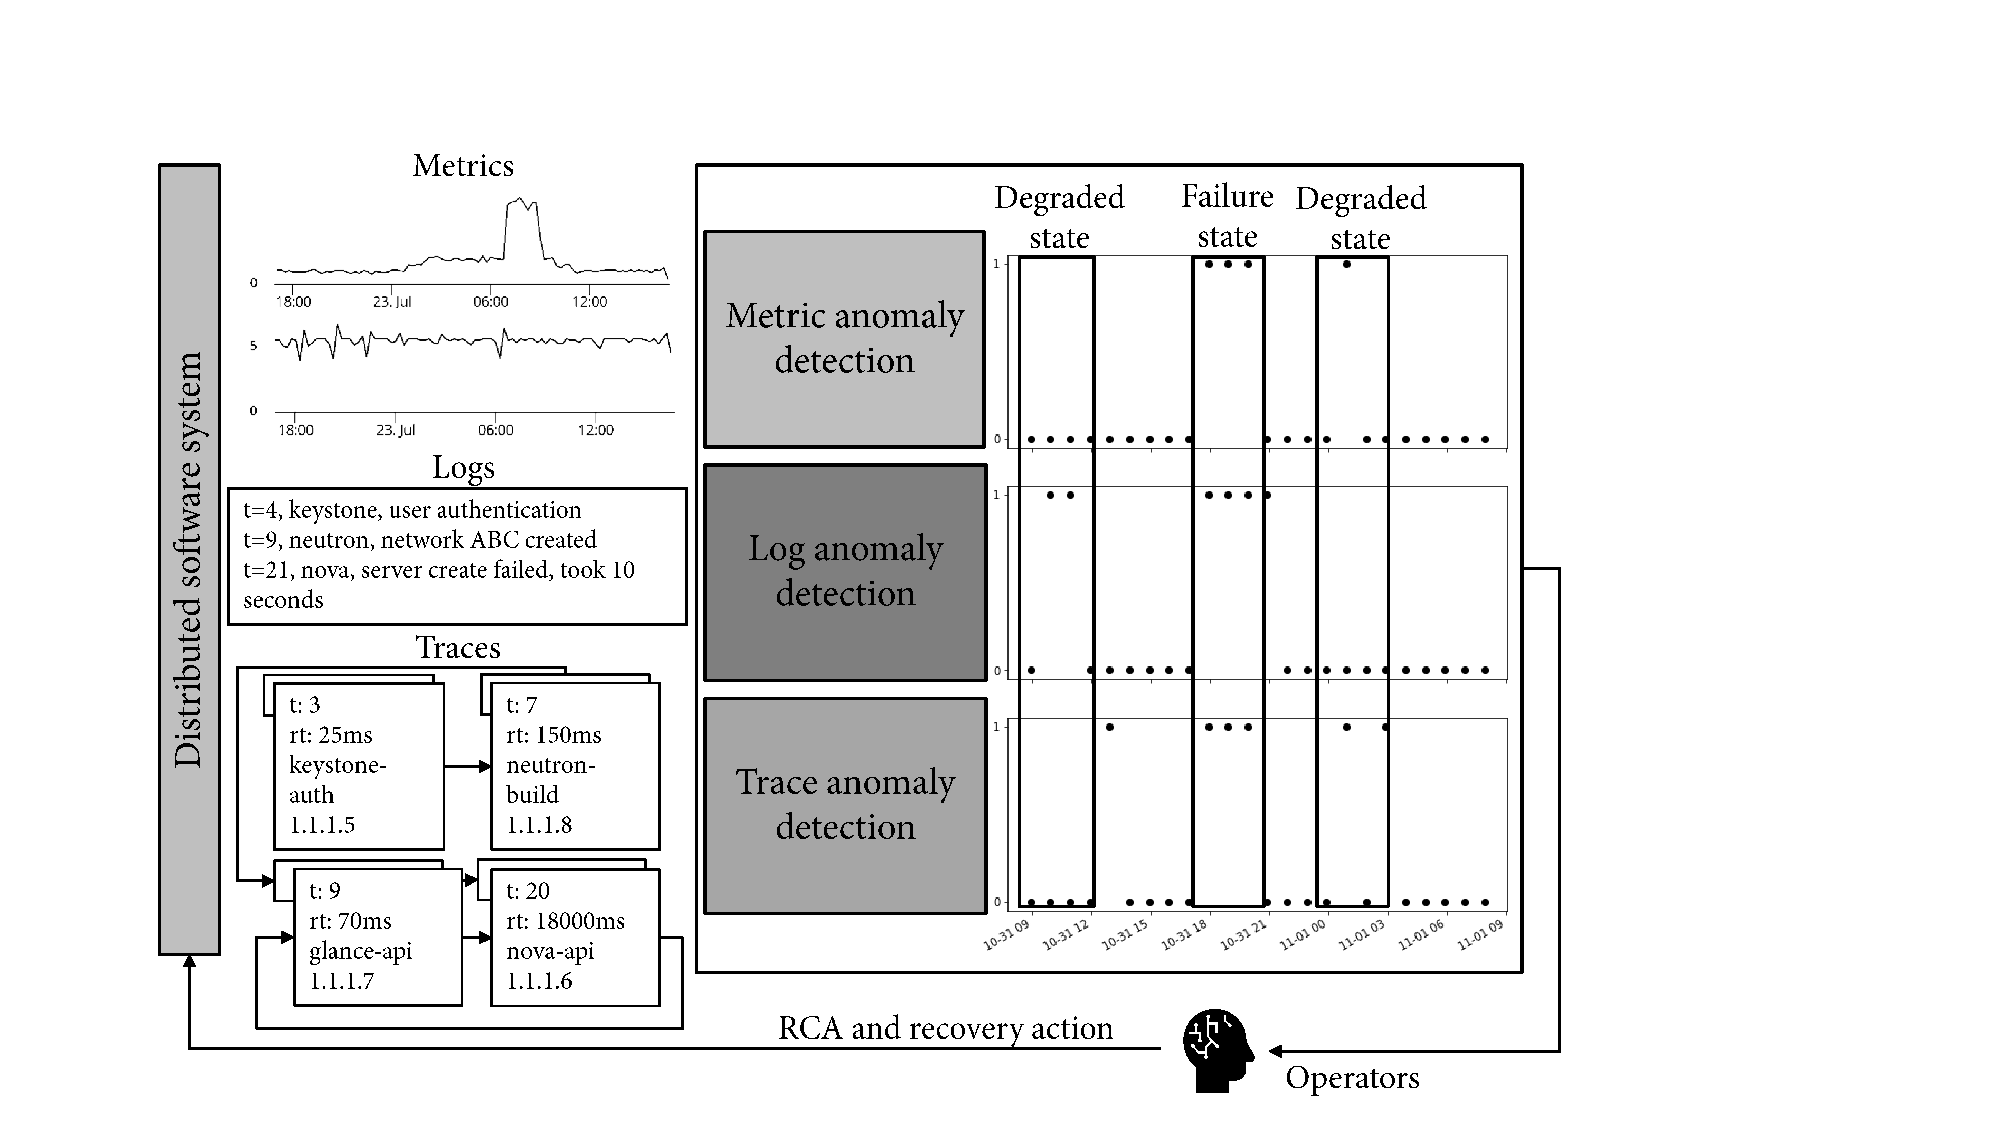
\includegraphics[width=1.0\textwidth]{gfx/chap7/solution_overview.pdf}}
\caption{Triano overview.}
\label{fig:Triano}
\end{figure}

\section{\textit{Triano}: integration of the anomaly detectors}
To address the problem of detection of complex anomalies, we introduce a rule-based integration of the detectors, denoted as Triano (see Figure~\ref{fig:Triano}).

We consider three trained anomaly detectors, presented in the previous chapters, $f_m(\mathbf{x_m})$, $f_l(\mathbf{x_l})$, and $f_t(\mathbf{x_t})$ for the metrics, logs, and traces, respectively. The input data in (1) $f_m(x_m)$ are a time series representing a system metric $\mathbf{x_m}={x_m^{w_m}, x_m^{w_m}, \dots, x_m^{w_m}}$, where $w_m$ is the window size, in (2) $f_l(x_l)$ are a system log message $\mathbf{x_l}={x_l^1, x_l^2, \dots, x_l^m}$, where $x_l^i$ are $d-$dimensional representations of the words in the log message and $m$ is the number of words, and in (3) $f_t(x_t)$ are a trace $\mathbf{x_t} = {x_t^1, x_t^2, \dots, x_t^k}$, where $x_t^i$ is a span and $k$ is the number of spans in the  trace. 

Each of the separate methods for anomaly detection in metrics, logs, and traces outputs its predictions, either 0 (normal) or 1 (anomaly), in the following format.

\begin{itemize}
    \item Metano, the metric anomaly detector $f_m(\mathbf{x_m})$, outputs \textit{(start time, end time, prediction, description}. The start and end time are the timestamps of the start and end of the window from the metric time series, while the prediction and description are related to the state of the system (normal or anomalous) and recognized anomaly pattern, as presented in~\autoref{ch:metrics}, respectively.
    \item Logsy, the anomaly detection method for log data $f_l(\mathbf{x_l})$, outputs \textit{(timestamp, prediction)} whether the observed log message is normal or anomalous, as presented in~\autoref{ch:logs}.
    \item Tracy, the anomaly detection method for trace data $f_t(x_t)$, outputs \textit{(start time, end time, prediction)} where the start and end times are the timestamps of the start and end of the analyzed trace, as presented in~\autoref{ch:traces}, respectively.
\end{itemize}

On top of the outputs of the anomaly detection methods, a time window $w$ is utilized to aggregate the predictions for a final decision, whether a possible anomaly exists in the observed system. Formally, the final output at a time $t$ is $g_t(f_m, f_l, f_t, w)$, which  is 0 or 1. As we observe different frequencies of predictions, first, the data from all data sources are aligned according to the start of the trace. 

An example of forming the final prediction is described. The tracing data contain information about multiple services, and thus the trace anomaly detector is prioritized. If this method reports an anomaly, the result is an anomaly is present. If anomaly is not present in the traces, logs are checked (log anomaly detector). If the log module does not generate an anomaly, the metric module is consulted. However, as depicted in Figure~\ref{fig:Triano}, the  approach is modular and any improvement in each of the detectors will improve the overall framework. Moreover, it enables flexibility of assessments of the order of the data sources, as the operator may have an additional knowledge on the type of anomalies that may arise in the system of interest. The knowledge can originate from either experience or availability of other informative sources such as source codes and configuration files.

We additionally designed a more complex multimodal deep learning method for automatic integration, however there were only negligible differences to the rule-based approach (see~\autoref{appendixA}).

\section{Evaluation}
In this section, we analyze the performance of Triano against single methods. We describe the experimental testbed, data, three anomaly cases, and evaluation. 

\begin{figure}[!htbp]
\centerline{\includegraphics[width=1.0\textwidth]{gfx/chap7/testbedTriano.pdf}}
\caption{Experimental testbed.}
\label{fig:Trianotestbed}
\end{figure}

\subsection{Experimental testbed}
For the generation of the data, we deployed an OpenStack~\cite{ShrivastwaOpenstack} testbed based on a microservice architecture running in a dockerized environment denoted as Kolla-Ansible~\cite{kollaansible}.
OpenStack is a cloud operating system, which controls large pools of computing, storage, and networking resources throughout a data center. All of them are managed and provisioned through APIs with common authentication mechanisms.
The experimental testbed is shown in Figure~\ref{fig:Trianotestbed}. For the generation of the data, it consists of one control node and four compute nodes. It was deployed on bare-metal nodes of a cluster. Each node has a RAM of 16 GB, three 1-TB disks, and two 1-Gbit Ethernet NICs. Three hard disks were combined to a software RAID 5 for data redundancy.

To generate user workload and inject faults into the system, we used Rally\cite{rally}. To evaluate the approach in scenarios close to real-world workloads, we used a series of user actions: create user -> create image -> create network -> start VM -> stop VM -> delete VM -> delete network -> delete image -> delete user. 

For monitoring and data collection, we utilized Prometheus for the metric data~\cite{turnbull2018monitoring}. Elasticsearch, Logstash, and Kibana (ELK) were used to aggregate logs from all services running across the physical nodes. To export logs from Elasticsearch into CSV, a CLI tool, es2csv, was utilized. To collect the traces, we utilize OSProfiler~\cite{openstack}, which is used by all OpenStack projects and their Python clients to generate traces. It generates one trace per request. 

To enable evaluation of the framework and methods, labeled data are required. Different data types require different labeling types. To label the data, we use the standard procedure of employing domain expert. (1) For traces, we consult a domain expert to label whether the trace is an anomaly. The trace may be either completed or not. We investigate its structure if it differs in many events, compared to the normal before providing it with a label. (2) For the logs, we analyze each log message using regex searches and label it to produce a labeled set of data. Anomalous log messages may appear outside the period of injection of anomalies. It is also important to label those instances. For the metrics, we perform the labeling in a similar manner. All models are trained by utilizing data from the time intervals when the system is in a normal state. 

\begin{table}[htbp]
\caption{Description of complex anomalies.}
\label{tab:complexanomalies}
\resizebox{\columnwidth}{!}{%
\begin{tabular}{cl}
\hline
Type            & \multicolumn{1}{c}{Description}                                                                                                                            \\ \hline
Network failure & \begin{tabular}[c]{@{}l@{}}Networking failure in the host node eliminated the access \\ to the host, leading to multiple failures (system hardware)\end{tabular} \\ \hline
Service update  & \begin{tabular}[c]{@{}l@{}}Configuration change in system A led to failures in A’s\\ calls to system B (deployment)\end{tabular}                           \\ \hline
Service failure & \begin{tabular}[c]{@{}l@{}}Failure in the message queue left several queues locked, \\ blocking messages (system software)\end{tabular}                    \\ \hline
\end{tabular}
}
\end{table}

\subsubsection{Anomaly scenarios}
To evaluate the combined approach against the single methods, we injected the anomalies described in Table~\ref{tab:complexanomalies}. 
The first considered anomaly is a network failure anomaly. This anomaly eliminates the access to a host, which leads to multiple failures. The second anomaly arises during deployment. Changes in configuration of system A led to failures in A calls to system B. We resolve this problem with deployment with a correct configuration. The third anomaly is a service failure. The anomaly is injected into the message queue (MQ) and leaves several queues locked, which blocks the message flow. We resolve it by cleaning the queue and restarting the service. 

\subsection{Results}


\begin{table}[!t]
\caption{Network failure multi-source anomalies; log data.}
\label{tab:network:logs}
\resizebox{\columnwidth}{!}{%
\begin{tabular}{cl}
\hline
Type     & \multicolumn{1}{c}{Log message}                                                                                                                                                                                                                                                                                                                                                                                       \\ \hline
Normal   & \begin{tabular}[c]{@{}l@{}}L1. 130.149.249.132  POST /v2.1/os-server-external-events HTTP/1.1 status: 200 len: 582 time: 0.0948207. \\ L2. {[}instance: f2adf232-3c39-477f-af0c-db25c9e4b4d6{]} During sync\_power\_state the instance has a pending \\ task (spawning). Skip.\end{tabular}                                                                                                                           \\ \hline
Degraded & \begin{tabular}[c]{@{}l@{}}L1. DHCP configuration for ports \{'451c037f-83d7-4fa7-86df-0b8afdbab99c'\} is completed“. \\ L2. 130.149.249.132  GET /v2.0/ports?device\_id=3322a8e7 b233-4115-96e1-f98450f1c2d0 HTTP/1.1\\ L3. failed to flush the buffer. retry\_time=2  next\_retry\_seconds chunk=error\_class=Fluent::Plugin::\\ ElasticsearchOutput::RecoverableRequestFailure read timeout reached“.\end{tabular} \\ \hline
Failure  & \begin{tabular}[c]{@{}l@{}}L1. failed to flush the buffer. retry\_time=1  next\_retry\_seconds chunk error\_class=Fluent::Plugin::\\ connect\_write timeout reached“. \\ L2. Function “nova.servicegroup.drivers.db.DbDriver.\_report\_state’ run outlasted interval by 0.25 sec“.\end{tabular}                                                                                                                       \\ \hline
\end{tabular}
}
\end{table}


\begin{figure}[!t]
\centerline{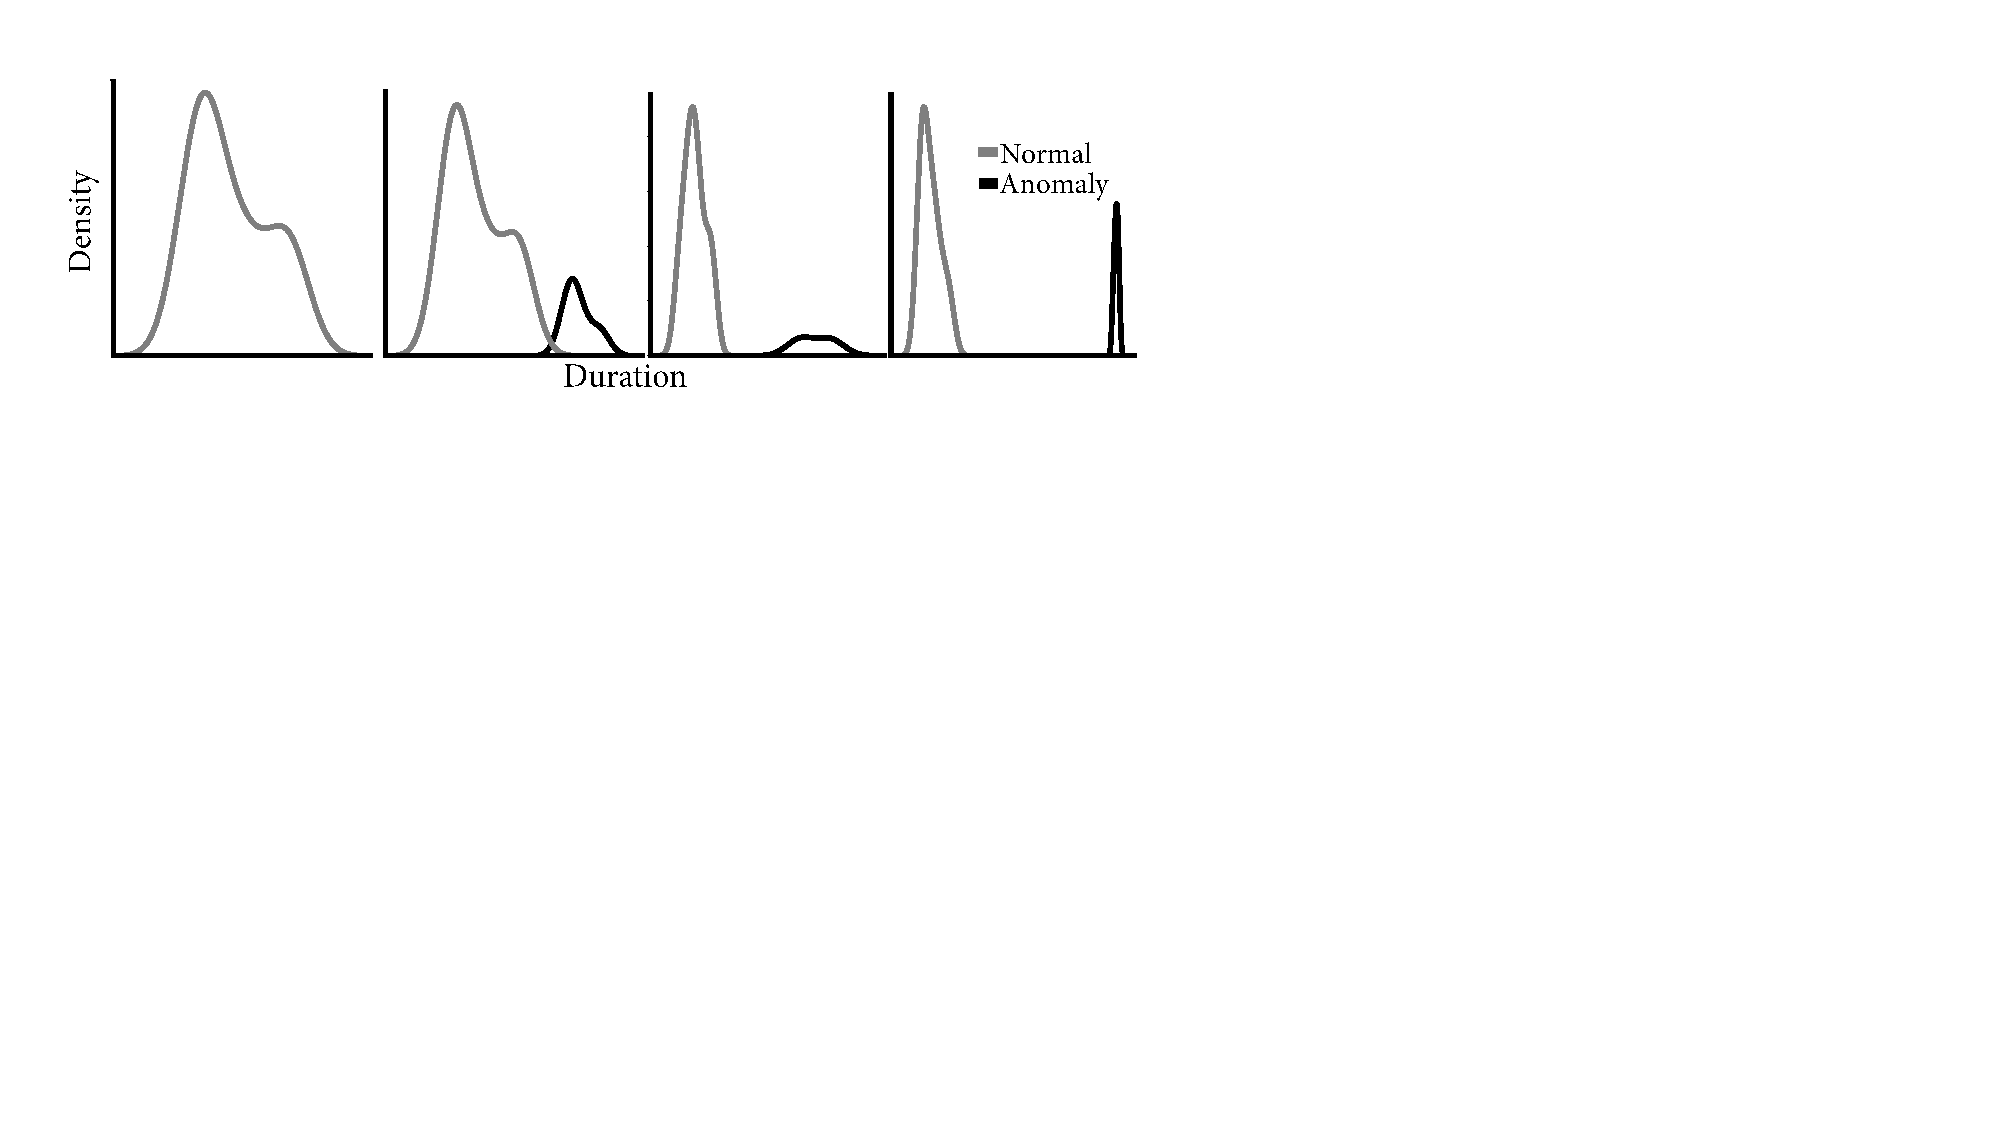
\includegraphics[width=0.9\textwidth]{gfx/chap7/metricsnetworkfailiure.pdf}}
\caption{Network failure multi-source anomalies. Normal metric distribution (left), two degraded states (middle), and failure state (right).}
\label{fig:network:metrics}
\end{figure}


\textbf{Network anomaly.}
Figures~\ref{fig:network:metrics} and \ref{fig:network:traces} show the metrics and traces, while Table~\ref{tab:network:logs} shows the logs, for the normal and abnormal executions of the operations. We carry out a simultaneous analysis of the three sources.


Figure~\ref{fig:network:metrics} shows the distributions of the response time durations during the normal and abnormal executions of the operations. The durations are represented as distribution plots of the duration of the normal (blue) and duration of the anomalous (orange) operations. During the normal state, the duration has a bimodal distribution, with one mode around 450 s and another mode around 500 s. We observe normal traces and logs. However, cross comparison of the durations during the small degradation (the second column for the metrics and first row for the traces) shows that the structures of the trace are similar, but the response times are different. Suspicious logs are not observed. This degradation is a problem reflected in the duration time, but not in other modalities. Hence, the duration serves as a good indicator of potential problems in the system. In this case, the metric method detects this anomaly, while the log and trace anomaly detectors are not able to detect this problem, as it is absent in the data. The combined approach detects this degradation problem as it is reflected in the metric data. On the contrary, if the decision is based solely on the logs or traces, the degradation will be missed out. This could lead to potential failures. 

\begin{figure}[!t]
\centerline{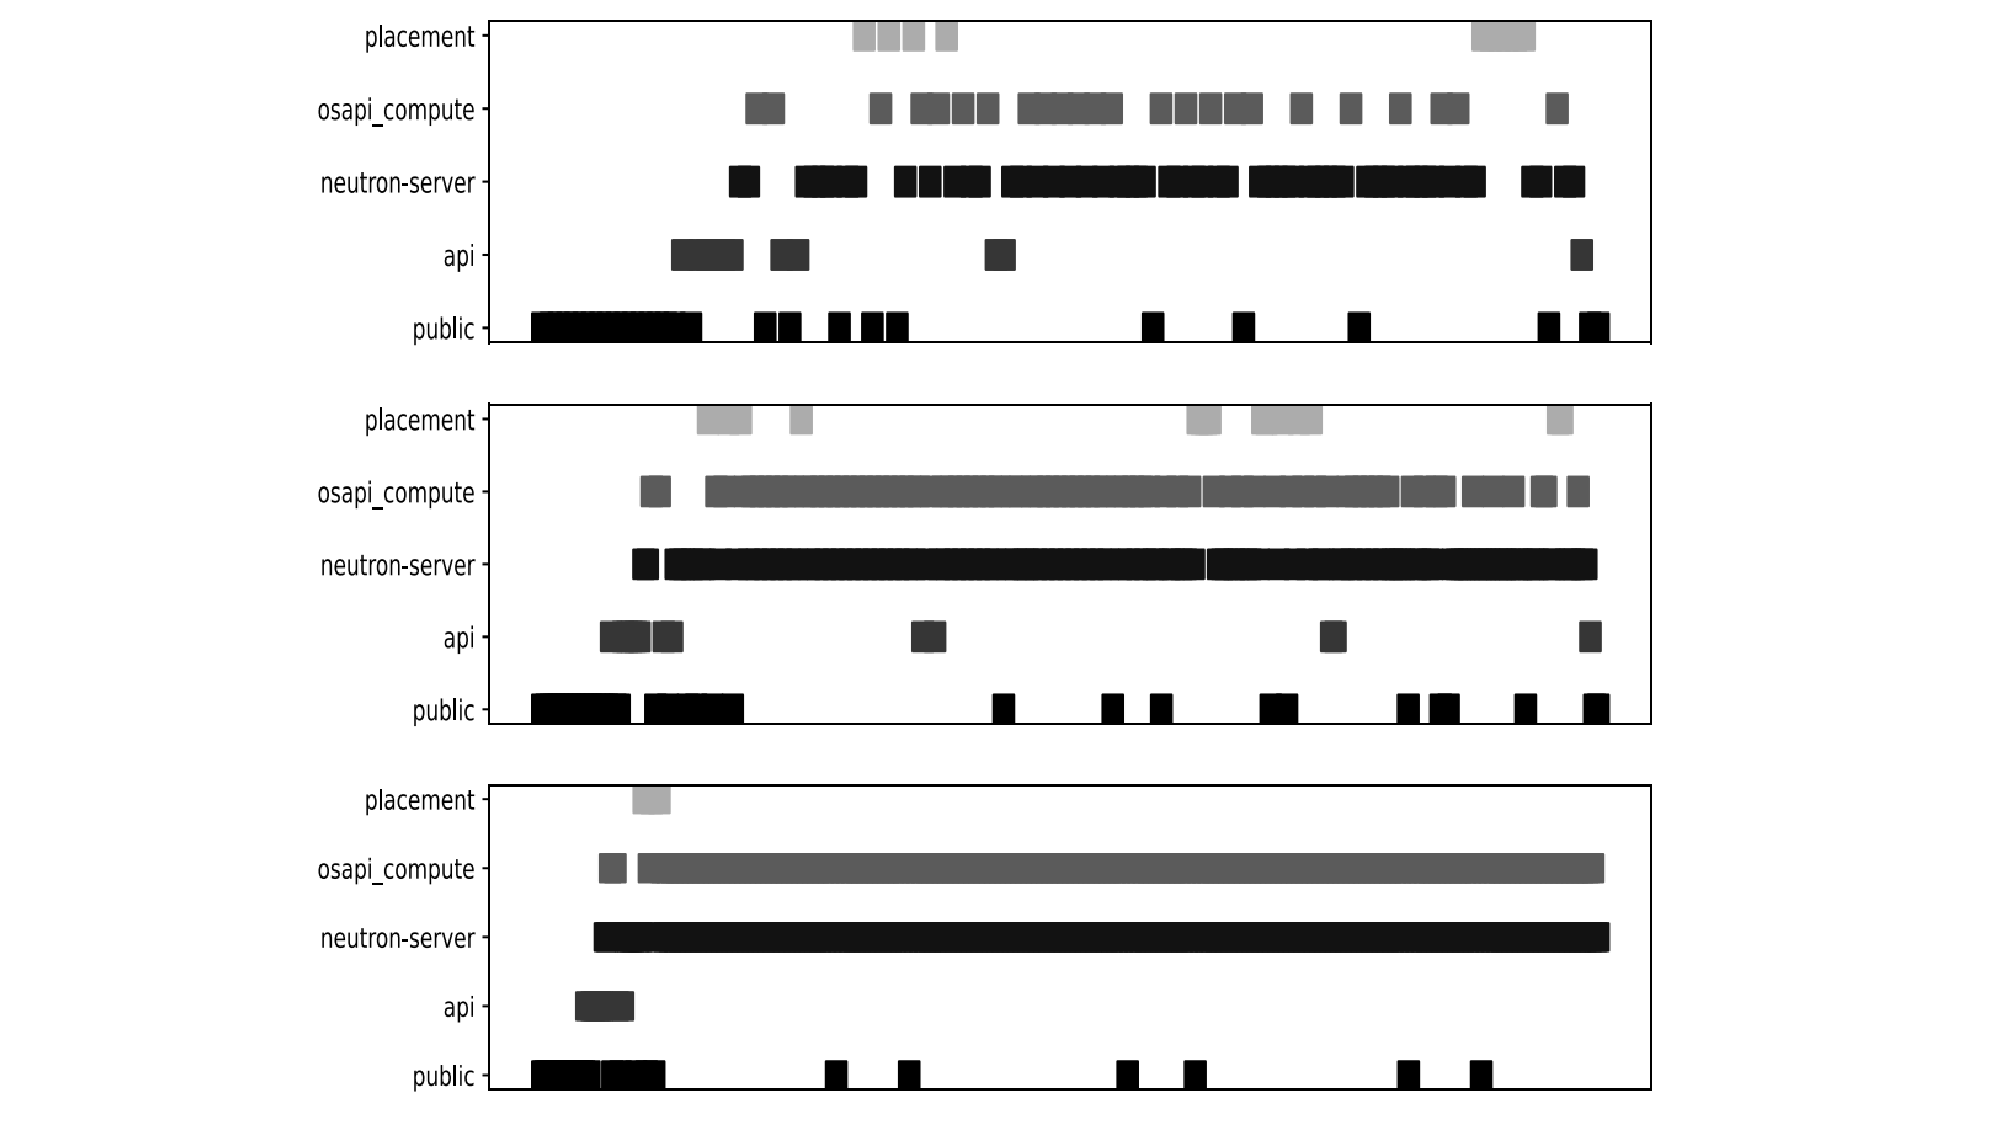
\includegraphics[width=0.9\textwidth]{gfx/chap7/tracesnetworkfailiure.pdf}}
\caption{Network failure multi-source anomalies. Normal trace (top), degradation (middle), and failure state (bottom).}
\label{fig:network:traces}
\end{figure}

Increasing the severity of the anomaly leads to a significant increase in the response time (the third column in Figure~\ref{fig:network:metrics}). In addition, the trace anomaly detector detects an anomalous trace and a structurally different trace is observed, while the logs are still unable to record anything. Triano detects the anomaly in the traces and metrics simultaneously. 

Finally, when the network of the host has failed, the trace cannot be completed. In addition, the response time is very large and timeout log messages appear. Furthermore, the trace anomaly detector and analysis of the scores per span show that the major issue is in nova-api (Figure~\ref{fig:network:traces}), which is hosted on the failed host. The Triano framework can detect all degraded and failed states. 



\begin{figure}[!b]
\centerline{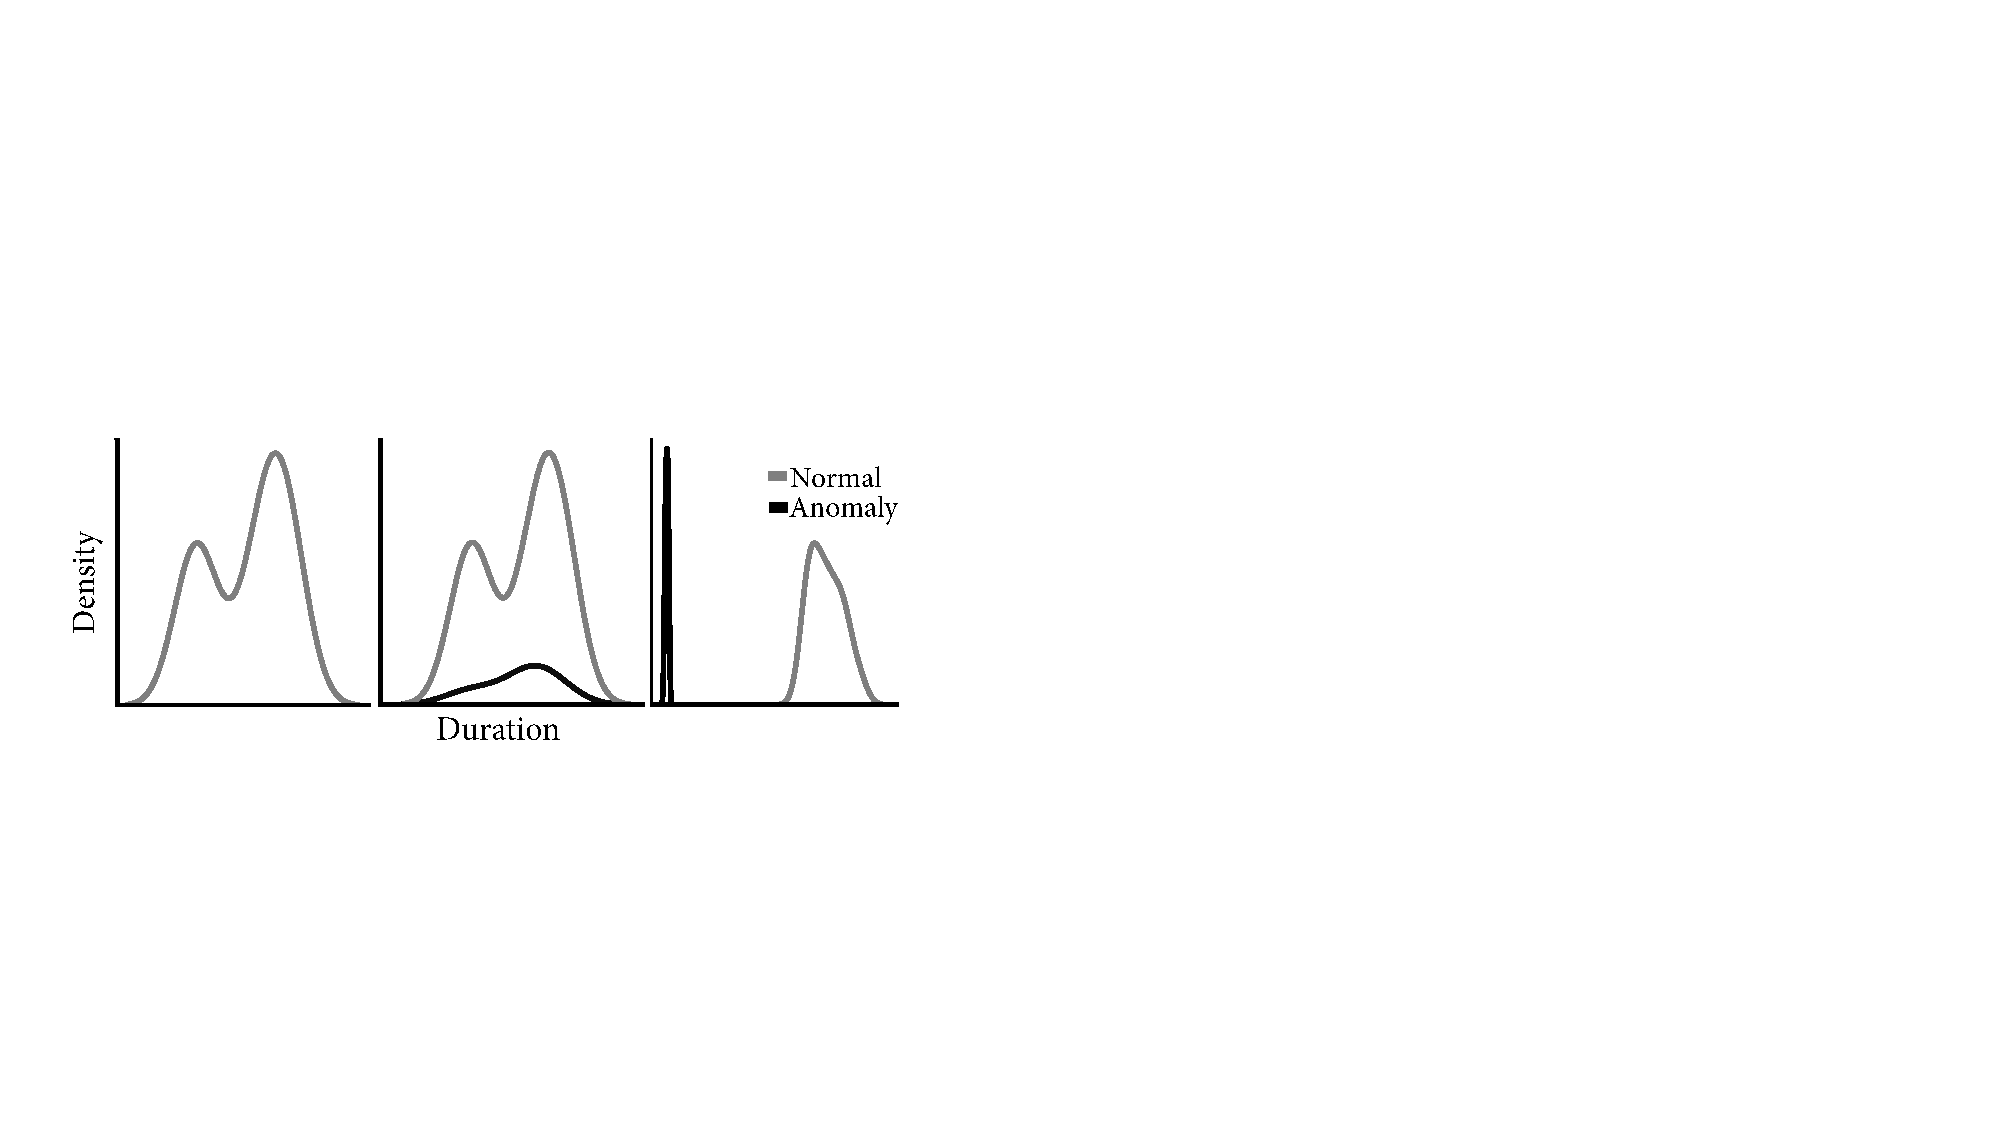
\includegraphics[width=0.9\textwidth]{gfx/chap7/serviceupdatemetrics.pdf}}
\caption{Service failure due to an update, multi-source anomalies, and metric data. Normal metric distribution (left), two degraded states (middle), and failure state (right).}
\label{fig:callservice:metric}
\end{figure}


\begin{table}[!t]
\caption{Service failure due to an update, multi-source anomalies, and log data.}
\label{tab:callservice:logs}
\resizebox{\columnwidth}{!}{%
\begin{tabular}{cl}
\hline
Type     & \multicolumn{1}{c}{Log message}                                                                                                                                                                                                                                                                                                                                                                                                            \\ \hline
Normal   & \begin{tabular}[c]{@{}l@{}}L1. {[}instance: 5d616cd-5689-44a0-8466-cf9290bff684{]} Instance spawned successfully. \\ L2. 130.149.249.132 - - {[}28/Sep/2020 20:02:13{]} GET /v2/images HTTP/1.1  200 16916 0.028519.\end{tabular}                                                                                                                                                                                                          \\ \hline
Degraded & \begin{tabular}[c]{@{}l@{}}L1. Traceback (most recent call last):   File  /usr/lib/python3/dist-packages/eventlet/ \\ wsgi.py  line 597, \\ BrokenPipeError: {[}Errno 32{]} Broken pipe“. \\ L2. 0.6783.0 closing AMQP connection \textless{}0.6783.0“.\end{tabular} \\ \hline
Failure  & \begin{tabular}[c]{@{}l@{}}L1. A recoverable connection/channel error occurred, trying to reconnect: {[}Errno 104{]} \\ Connection reset by peer“. \\ L2. Error from libvirt while getting description of instance-00000199: {[}Error Code 42{]}\end{tabular}                                                                                                                              \\ \hline
\end{tabular}
}
\end{table}


\textbf{Configuration change in service A leads to a failure in service A calls to service B.}
Another common type of anomaly appears when a change in the configuration file of one service A leads to failures in the service A call for service B. Different such cases exist. The results of the analysis of this scenario are presented in Figure~\ref{fig:callservice:metric}, Figure~\ref{fig:callservice:traces}, and Table~\ref{tab:callservice:logs}.

Such changes can appear in the configuration when all appears normal from the response time and trace perspectives. The center--top image shows that the durations for both normal and abnormal response times have an overlap in the distributions.
However, the log anomaly detector report problems. The degradation phase is present only inside the logs. 

Severe cases of this anomaly lead to a failure. The duration in this case is very small for the failed operations and the traces are out of order. In addition, anomalous log messages exist.


\begin{figure}[!t]
\centerline{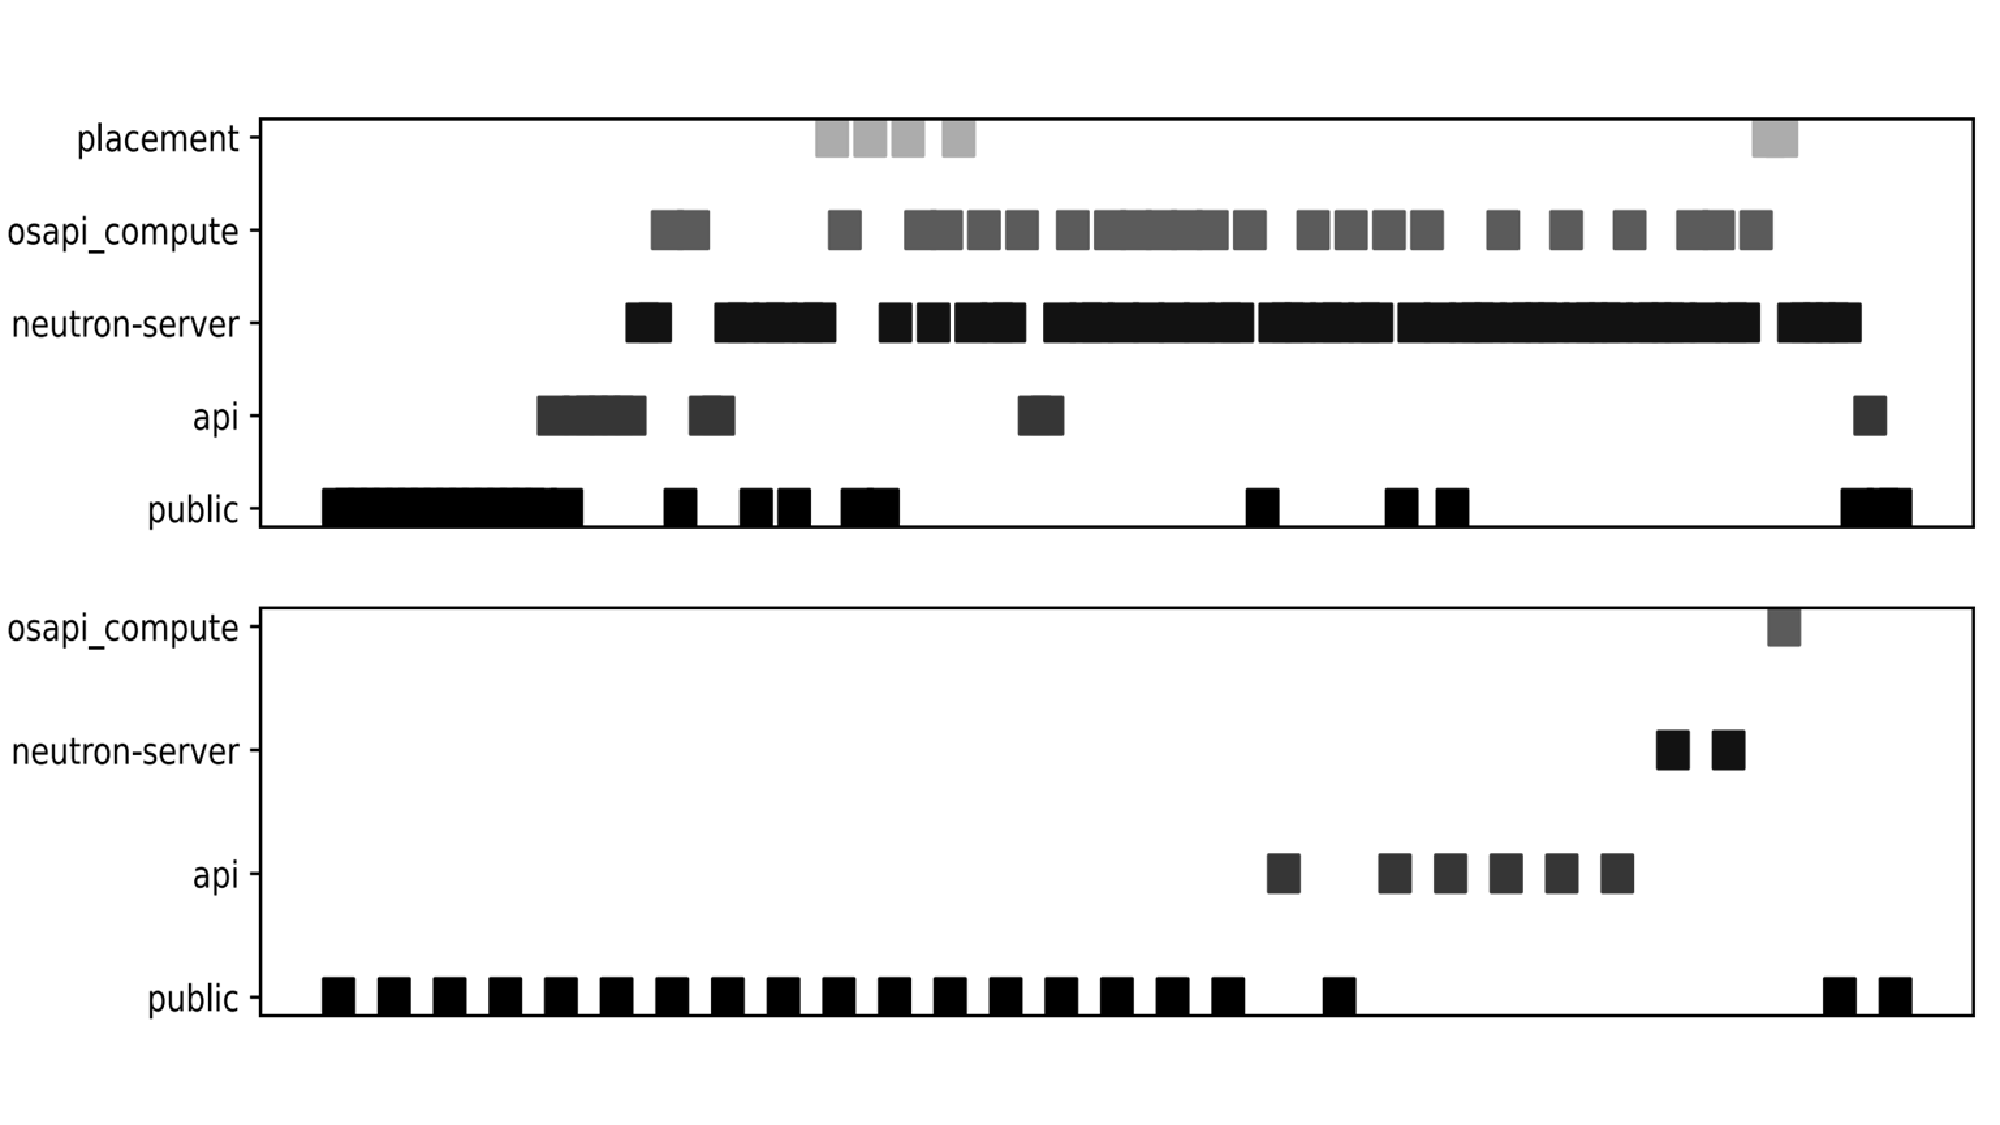
\includegraphics[width=0.9\textwidth]{gfx/chap7/serviceupdatetraces.pdf}}
\caption{Service failure due to an update, multi-source anomalies, and trace data. Normal state (top) and failure state (bottom).}
\label{fig:callservice:traces}
\end{figure}









\textbf{Failure in MQ left several queues locked, blocking messages}
The results of the analysis of this scenario are presented in Figure~\ref{fig:service:metric}, Figure~\ref{fig:service:trace}, and Table~\ref{tab:service:logs}.

A limitation in the MQ, not exposed during testing, can bring it to a degraded state, for example, due to an increased traffic. During this period, the times needed for execution of an operation during the normal and abnormal periods may not differ significantly, as shown in Figure~\ref{fig:service:metric}. The middle image shows that the response times for both normal and abnormal behaviours have an overlap in the distributions. Although insignificant, as in the previous case, it can lead to FP reported by the metric module. The trace is not affected as the requests are executed. In this scenario, the log messages report problems in the form of "Recoverable Connection Error". 

The failure state has a similar structure to those in the previous two use cases. The duration in this case is very small for the failed operations and the traces are completely out of order. In addition, anomalous log messages in the form of "timeouts" exist. The neutron cannot perform specific requests. The queues are locked and all messages are blocked. 



\begin{table}[!htbp]
\caption{Anomaly in the MQ; log data.}
\label{tab:service:logs}
\resizebox{\columnwidth}{!}{%
\begin{tabular}{cl}
\hline
Type     & \multicolumn{1}{c}{Log message}                                                                                                                                                                                                                                                                                                                                                                                                                  \\ \hline
Normal   & \begin{tabular}[c]{@{}l@{}}L1. "130.149.249.132   GET /v2.0/ports?device\_id=3be3c024-d97e-448a-a30d-015e82571606  HTTP/1.1\\ L2. "Security group member updated \{'cad0f51f-3235-4ec2-9b8a-97761195cc5c’\}”.\end{tabular}                                                                                                                                                                                                                       \\ \hline
Degraded & \begin{tabular}[c]{@{}l@{}}L1. AMQP server on 130.149.249.132:5672  is unreachable: \textless{}RecoverableConnectionError: unknown error\textgreater{}.\\ Trying again in 1 seconds.: amqp.exceptions.RecoverableConnectionError\\ L2. AMQP server on 130.149.249.132:5672 is unreachable: Too many heartbeats missed. Trying again\\ in 1 seconds.: amqp.exceptions.ConnectionForced: Too many heartbeats missed“.\textbackslash{}\end{tabular} \\ \hline
Failure  & \begin{tabular}[c]{@{}l@{}}L1. AMQP server on 130.149.249.132:5672 is unreachable: Too many heartbeats missed. \\ Trying again in 1 seconds.: amqp.exceptions.ConnectionForced: Too many heartbeats missed“. \\ L2. AMQP server on 130.149.249.132:5672 is unreachable: timed out.\\ Trying again in 8 seconds.: socket.timeout: timed out“.\end{tabular}                                                                                        \\ \hline
\end{tabular}
}
\end{table}


\begin{figure}[!t]
\centerline{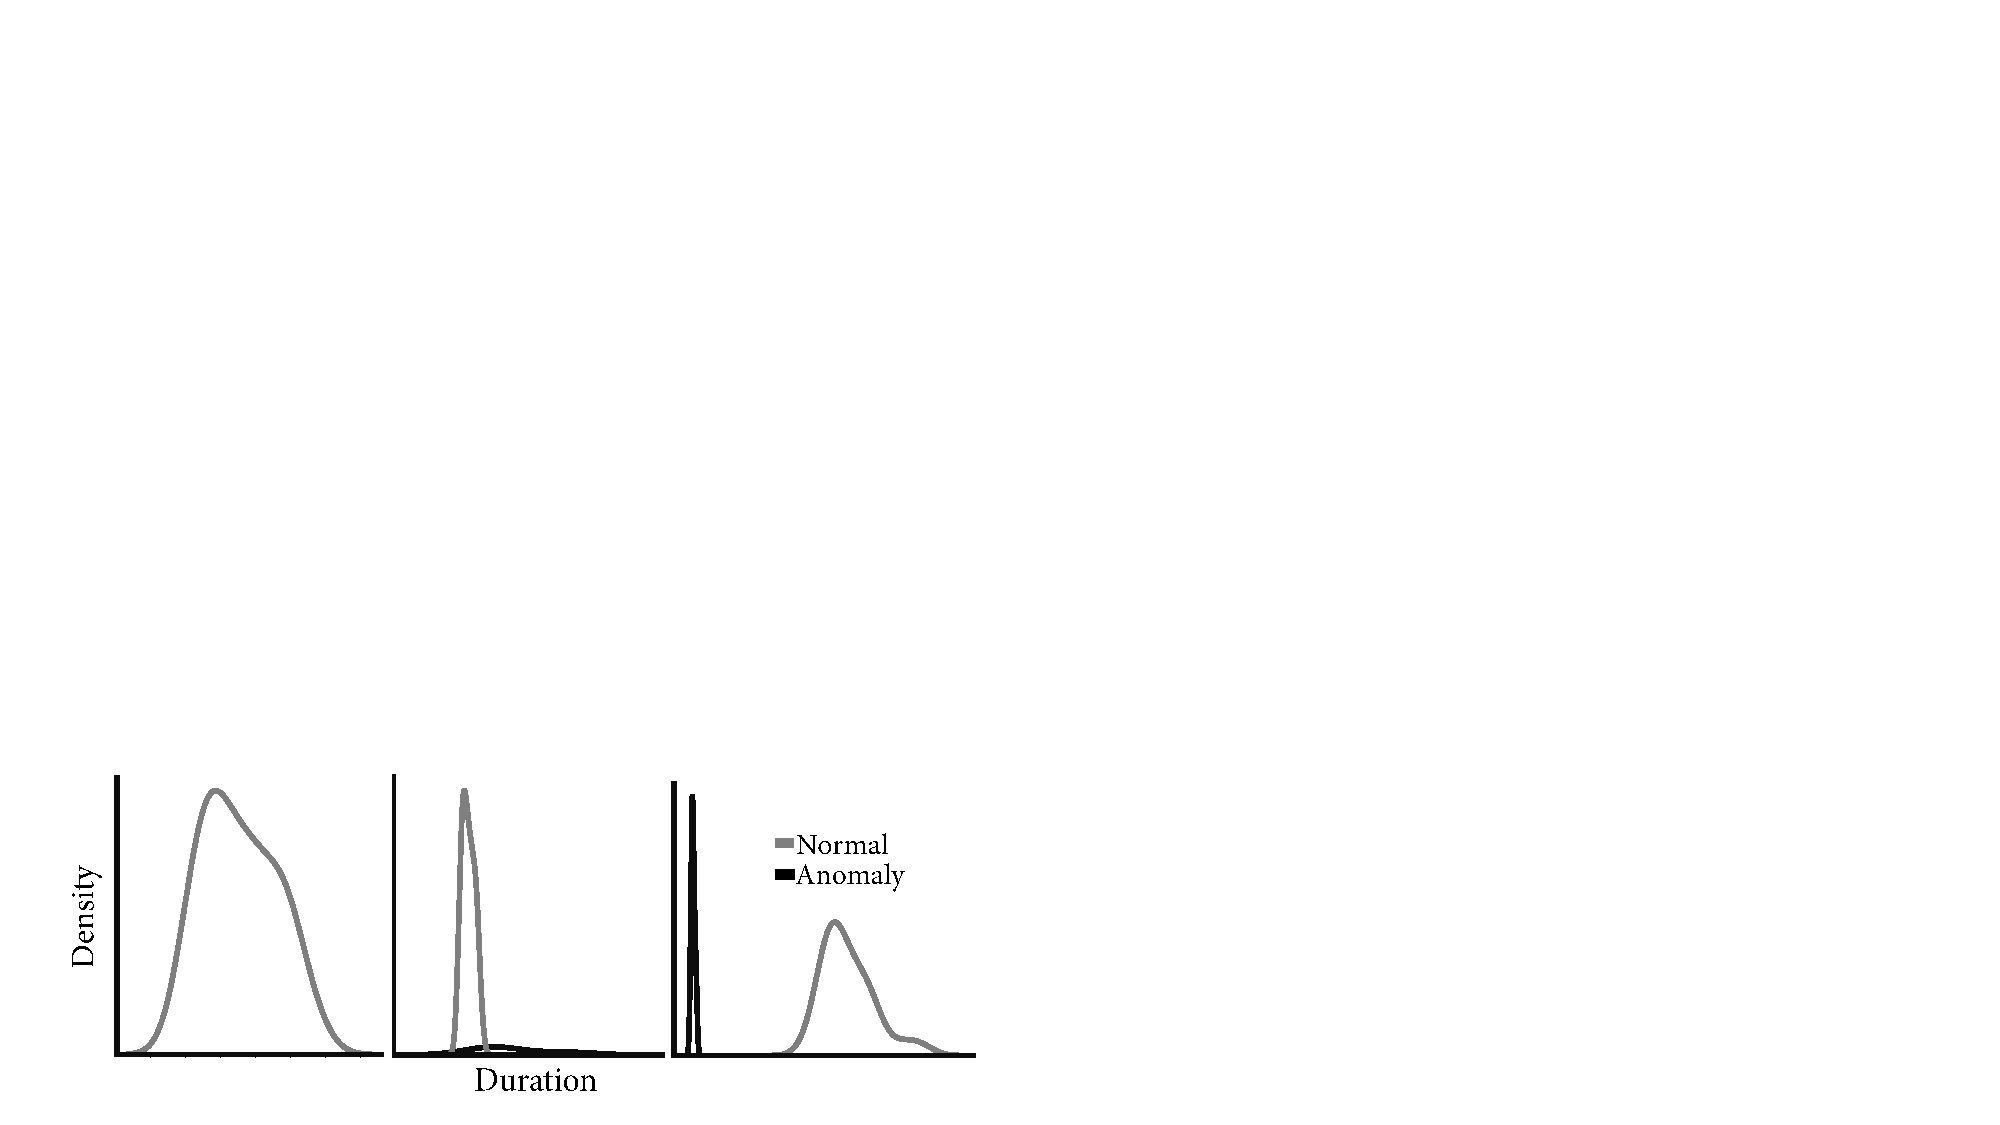
\includegraphics[width=0.9\textwidth]{gfx/chap7/servicefailiuremetrics.pdf}}
\caption{Anomaly in the MQ; metric data. Normal (left), degraded (middle), failure (right).}
\label{fig:service:metric}
\end{figure}

\begin{figure}[!t]
\centerline{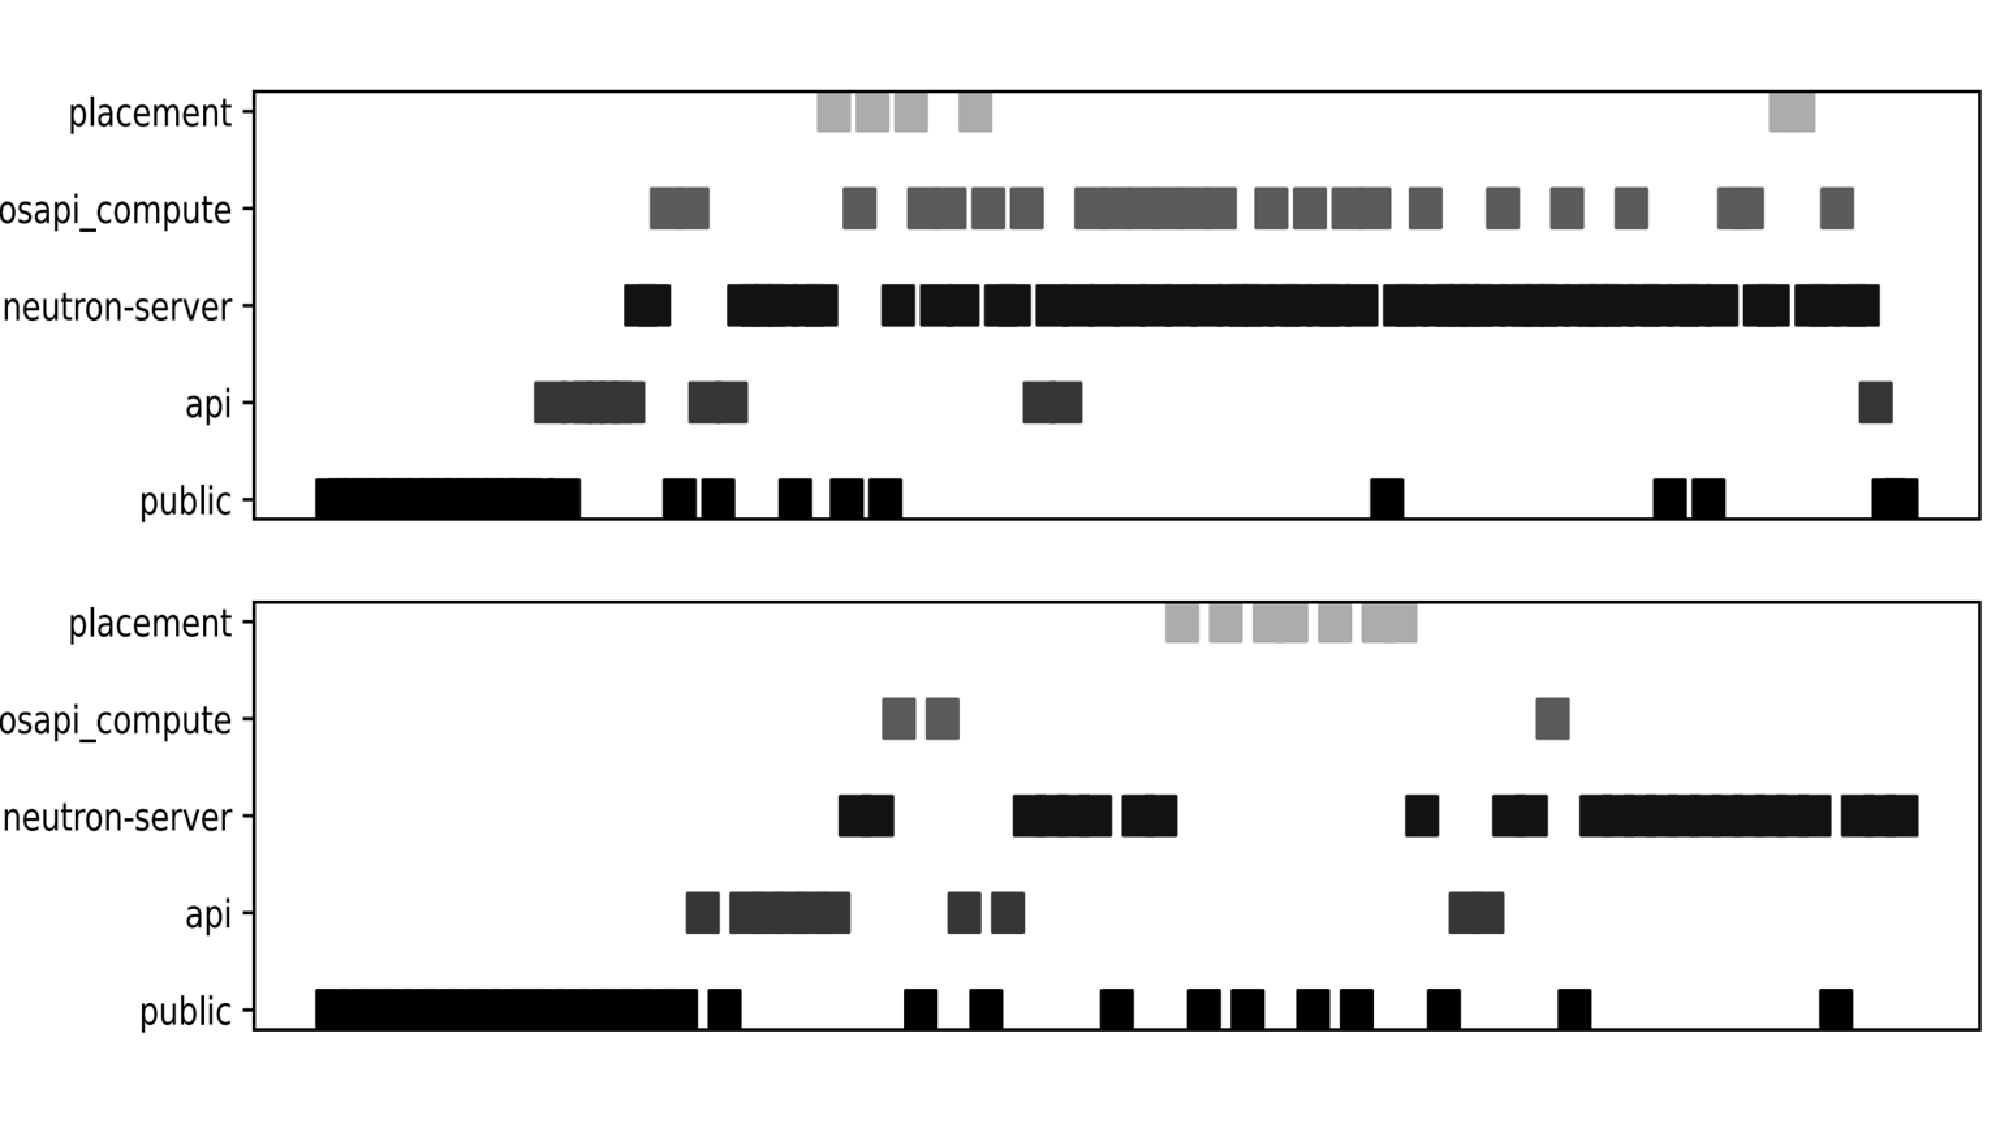
\includegraphics[width=0.9\textwidth]{gfx/chap7/servicefailiuretraces.pdf}}
\caption{Anomaly in the MQ; trace data.}
\label{fig:service:trace}
\end{figure}

\newpage

\subsection{Results summary}
Table~\ref{tab:rescomplex} shows the three scenarios of complex anomalies presented in the previous section. For each observability component, the two states (degradation D, failure F) are shown. Some of the anomalies are not reflected in all three modalities, while in some cases, they are reflected in all of them (mostly degraded-state anomalies). We denote the F1-scores of Metano (metrics), Logsy (logs), and Tracy (traces) with plus (+), if greater than 0.9, and minus (-) less than 0.1. This reflects if the method can successfully detect the anomaly in the particular case. From the table, it can be concluded that the methods can detect anomalies which are found in the data, and not detect anomalies which are hidden. For example, during the networking anomaly, the degradation phase in the system does not appear in the logs but appears in the traces. Thus, Logsy is not able to detect any anomaly, while Tracy manages to capture all of them. Similarly, the service update and service deployment anomalies during the degradation stage do not appear in the traces and metrics but appear in the logs.

\begin{table}[!t]
\caption{Results of the detection of the complex anomalies.}
\label{tab:rescomplex}
\resizebox{\columnwidth}{!}{%
\begin{tabular}{clcccc}
\hline
Type            & \multicolumn{1}{c}{Description}                                                                                                                            & Metrics (D,F) & Logs (D,F) & Traces (D,F) & Triano (D,F) \\ \hline
Network failure & \begin{tabular}[c]{@{}l@{}}Networking failure in the host node\\ eliminated the access to the host, leading \\ to multiple failures (system hardware)\end{tabular} & +  +   & 0  + & 0  +  & +  +  \\ \hline
Service update  & \begin{tabular}[c]{@{}l@{}}Configuration change in system A \\ led to failures in A’s calls to\\ system B (deployment)\end{tabular}                           & 0 +     & + +   & 0 +    & + +    \\ \hline
Service failure & \begin{tabular}[c]{@{}l@{}}Failure in the MQ \\ left several queues locked, \\ blocking messages (system software)\end{tabular}                    & 0 +     & + +   & 0 +    & + +    \\ \hline
\end{tabular}
}
\end{table}

Full observability implies a considerably higher probability to detect all anomalies than that in the single-model scenario. To successfully address the problem of complex anomalies, full observability of the system is required.

\newpage

\section{Related work}
A limited number of studies in the academia that combined multiple data sources for anomaly detection in distributed systems exist. Most claimed solutions are from the industry, where companies provide various services for automation in the IT domain. These solutions are predominantly patented. 

Farshchi et al.~\cite{farshchi2018metric} addressed the problem of monitoring cloud application operations through log and metric analyses. Their contributions include a novel approach that assists in finding the subset with the most relevant monitoring metrics. It further includes employing those metrics for the reliable assurance of the correct execution of sporadic cloud operations, particularly in staged upgrading of clusters of VMs. The core of the approach is a domain-agnostic regression-based correlation analysis technique that correlates operations’ event logs and resource metrics. Based on this correlation, it can identify which monitoring metrics are significantly affected by operation’s activities and how. In Weber et al~\cite{weber2016dependability}, the authors proposed the POD framework, which targets the dependability of cloud application deployment specifically. At the core, it uses cloud metrics and logs from operations
tools. During normal system behaviour of such operations processes, the framework collects logs and metrics. These are used in the offline training phase, where a process model for the operation from the logs is obtained through process mining techniques and human interaction. In the online phase, the framework uses current logs and metrics in combination with the created process model. They present two POD-Detection services for this purpose. First, the conformance checker tracks if the behavior and timing of the current execution is in line with the model. Second, assertion evaluation tracks the effects of the current execution on the metrics, and uses hand-coded additional assertions to check against the cloud API if process steps have the desired effect. If any errors are detected, diagnosis and recovery are triggered. This approach is related to Triano, however, it models the correlation between the operational logs and metrics, whereas in Triano, we consider metrics, logs, and traces, independently. Moreover, the POD framework aims to detect process anomalies, where Triano is focused on analyzing various data sources on more granular level. 

In our work on multimodal anomaly detection~\cite{nedelkoski2020jointmodalities}, following previous studies from Ikeda et al.~\cite{Japan}, we utilized the joint representation from the distributed traces and system log data for the task of anomaly detection in distributed systems. We found that this approach of learning the joint information of logs and traces into one more complex model yields insignificant differences when compared to the independent detectors.

The Splunk~\cite{zadrozny2013big} software platform allows its users to analyze and visualize the data gathered by the IT components. Data are collected from various sources and indexed. The indexed data are then presented in a series of events, from where they can be searched as well as viewed. Key features of Splunk include searching from the data, calculating metrics, predictions, event retrieving, alerting whenever a configured search condition is met, and reporting. This allows to save searches as reports. The user can later add them to dashboards and even schedule them for generating alerts under particular conditions.

AppDynamics~\cite{bansal2015automatic,bansal2015monitoring,bansal2015conducting} is an application performance management and IT operation platform, which provides automated anomaly detection. From the publicly available information, AppDynamics utilizes thresholds on KPIs and comparisons to baselines to perform the anomaly detection.

Moogsoft~\cite{tee2016system,tee2017alert} is a provider of AIOps solutions. In the Moogsoft AI platform, real-time data are collected through various sources and the events associated with the data are correlated. The obtained insights are thereafter shared with operation teams, which help improve the mean time to repair. The main features include real-time monitoring of systems, providing alerts as soon as they are detected based on setting thresholds for KPIs and generating accurate incident reports that help the recovery of the system.

Loom System is an AIOps solution, which helps the prediction and elimination of the issues that arise while migrating to clouds. The AIOps solution by Loom systems is capable of preventing IT issues before customers are affected. Its operation can be described as follows. Data Collection: Log and metric data are collected from various sources and are later divided according to their purposes. The collected data are classified with the required measurement methods.
Anomaly Detection: With machine learning algorithms, the approach sets a certain measurement in real time to detect the emerging issues at the initial stages. Root Cause Analysis: With the help of cognitive reasoning, cross-application issues are detected, providing information about the digital environment.

Other similar solutions from the industry are listed in Gartner reports~\cite{gartnermarketguide,gartnerinc}.

In the literature, to the best of our knowledge, we rarely identify solutions for unsupervised anomaly detection of metrics, logs, and traces as fundamentally complementary data sources in one framework. 


\section{Chapter summary}
In this chapter, we utilized the previously described methods in \autoref{ch:metrics}, \autoref{ch:logs}, and \autoref{ch:traces} to perform anomaly detection. Through the empirical evaluation, we showed that the proposed approach detects the various complex anomalies that manifest in distributed software systems in unpredictable manners, e.g., propagation of the anomaly between components of the system or hidden from specific observability tools. Owing to the modularity of the approach, improvements in the anomaly detection methods for metrics, logs, and traces lead to overall improvements. In addition, we designed and evaluated a method that learns joint representations from logs and traces. We showed that even by increasing complexity to process the data types in one model, the multimodal method exhibits negligible differences to independent detectors. A reason for such behavior can be that the data sources as they are (e.g., logs and traces) they contain orthogonal information. Lastly, through discussions we demonstrated that full observability increases the chances of timely detection of broader spectrum of anomalies.


